\chapter{Teoría de Grafos}

\section{Conceptos fundamentales}

\subsection{Definiciones básicas}

\begin{definicion}
Una \textbf{familia enumerable} es una colección enumerable de objetos iguales o diferentes.
\begin{itemize}
  \item El mayor número $p$ de elementos iguales en una familia enumerable le llamamos \textbf{grado de multiplicidad}.
  \item Una familia enumerable con $p = 1$ se llama \textbf{conjunto}.
  \item En lo que sigue, consideraremos solo familias finitas.
  \item El conjunto de partes de $X$ será denotado $\mathcal{P}(X)$.
  \item $\mathcal{P}_k(X) = \{U \in \mathcal{P}(X) \mid |U| = k\}$.
  \item La potencia cartesiana $X^k$ es el conjunto de todas las $k$-uplas ordenadas $(x_1, x_2, \ldots, x_k)$ donde $x_i \in X$, $1 \leq i \leq k$, $1 \leq k \leq |X|$.
\end{itemize}
\end{definicion}

\begin{definicion}
Un \textbf{grafo} es una estructura $G = (N, A)$ donde $N$ es un conjunto finito y $A$ es una familia cuyos elementos (no vacíos) son definidos en función de los elementos $v$ de $N$, en dos formas posibles:

\begin{enumerate}
  \item Si la familia $A$ de grado de multiplicidad $p$ fuera tal que sus elementos $a \in \mathcal{P}(N)$, $G$ será llamado un \textbf{$p$-hipergrafo no orientado}.
  \item Si la familia $A$ de grado de multiplicidad $p$ es constituida por pares de elementos no vacíos de $\mathcal{P}(N)$ de la forma $a_i = (a_i^-, a_i^+)$, $G$ será llamado un \textbf{$p$-hipergrafo orientado}.
\end{enumerate}

\begin{itemize}
  \item Los elementos de $N$ son llamados \textbf{nodos} (o vértices) y el valor $n = |N|$ es el \textbf{orden} de la estructura.
  \item La familia $A$ puede ser entendida como una relación o conjunto de relaciones de adyacencia cuyos elementos son llamados en general \textbf{conexiones}; en particular, en las estructuras no orientadas las $a \in A$ son conocidas como \textbf{aristas} y en las orientadas como \textbf{arcos}.
  \item Dos nodos que participan de una conexión son llamados \textbf{adyacentes}.
  \item Al valor $m = |A|$ lo llamaremos el \textbf{tamaño} del grafo.
  \item Si $m = 0$, el grafo es llamado \textbf{trivial}.
  \item La representación dinámica de un grafo, también llamado grafo (confusión semiintensional), es obtenida asociando a cada nodo un punto o una pequeña área delimitada por una frontera, y a cada conexión un diseño capaz de representar la forma de asociación de los nodos que involucra la conexión.
\end{itemize}
\end{definicion}

\begin{ejemplo}
Los siguientes gráficos representan aristas o arcos. (Ver Figura~\ref{fig:aristas-arcos}.)
\end{ejemplo}

\begin{figure}[htbp]
\centering
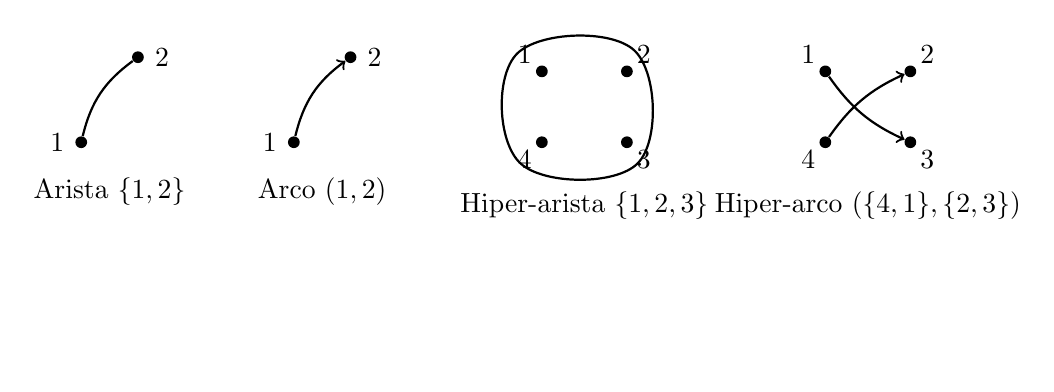
\begin{tikzpicture}[scale=0.9, every node/.style={circle, fill=black, inner sep=1.5pt}]
% Arista
\begin{scope}[xshift=0cm]
\node[label=left:{1}] (a1) at (0,0) {};
\node[label=right:{2}] (a2) at (0.8,1.2) {};
\draw[thick] (a1) to[bend left=20] (a2);
\node[fill=none] at (0.4,-0.7) {Arista $\{1,2\}$};
\end{scope}

% Arco
\begin{scope}[xshift=3cm]
\node[label=left:{1}] (b1) at (0,0) {};
\node[label=right:{2}] (b2) at (0.8,1.2) {};
\draw[thick,->] (b1) to[bend left=20] (b2);
\node[fill=none] at (0.4,-0.7) {Arco $(1,2)$};
\end{scope}

% Hiper-arista
\begin{scope}[xshift=6.5cm]
\node[label=above left:{1}] (c1) at (0,1) {};
\node[label=above right:{2}] (c2) at (1.2,1) {};
\node[label=below left:{4}] (c4) at (0,0) {};
\node[label=below right:{3}] (c3) at (1.2,0) {};
\draw[thick] plot [smooth cycle, tension=0.7] coordinates {(-0.35,1.25) (1.3,1.3) (1.35,-0.3) (-0.3,-0.3)};
\node[fill=none] at (0.6,-0.9) {Hiper-arista $\{1,2,3\}$};
\end{scope}

% Hiper-arco
\begin{scope}[xshift=10.5cm]
\node[label=above left:{1}] (d1) at (0,1) {};
\node[label=above right:{2}] (d2) at (1.2,1) {};
\node[label=below left:{4}] (d4) at (0,0) {};
\node[label=below right:{3}] (d3) at (1.2,0) {};
\draw[thick,->] (d1) to[bend right=15] (d3);
\draw[thick,->] (d4) to[bend left=15] (d2);
\node[fill=none] at (0.6,-0.9) {Hiper-arco $(\{4,1\},\{2,3\})$};
\end{scope}
\end{tikzpicture}
\caption{Utilizaremos el término grafo para designar estructuras que posean conexiones con un máximo de dos nodos involucrados y, a menos que se indique lo contrario, con grado de multiplicidad igual a 1.}
\label{fig:aristas-arcos}
\end{figure}

\begin{observacion}
\begin{enumerate}
  \item[a)] Para $G = (N, A)$ un $p$-hipergrafo no orientado, en particular, si:
  \begin{itemize}
    \item Se verifica que todos los elementos de $A$ pertenecen a $\mathcal{P}_1(N) \cup \mathcal{P}_2(N)$; $G$ es llamado un \textbf{multigrafo} o \textbf{$p$-grafo no orientado}.
    \item $A$ fuese un subconjunto de $\mathcal{P}(N)$, $G$ será \textbf{1-hipergrafo no orientado} o \textbf{hipergrafo simple}.
  \end{itemize}
  \item[b)] Para $G = (N, A)$ un 1-hipergrafo orientado, en particular, si:
  \begin{itemize}
    \item Se tuviera $|a_i^-| = |a_i^+| = 1$ para todo $i$, $G$ se denominará \textbf{1-grafo orientado} o \textbf{dígrafo}.
  \end{itemize}
  \item[c)] Una conexión que tiene apenas un nodo es llamada \textbf{bucle} o \textbf{lazo}. En las estructuras no orientadas un lazo es un elemento de $\mathcal{P}_1(N)$ y en las orientadas, una $k$-upla de elementos iguales; en grafos orientados, un par ordenado de elementos iguales.
  \item[d)] Asociado a todo grafo orientado $G = (N, A)$ existe un grafo $G' = (N, A')$ en el cual todo arco $a' = (y, x)$ tiene en $A$ un arco correspondiente $a = (x, y)$. Al grafo $G'$ se le denomina el \textbf{dual direccional} de $G$.
\end{enumerate}
\end{observacion}

\begin{ejemplo}
A continuación se presentan diversos tipos de estructuras de grafo: 3-hipergrafo no orientado, 1-hipergrafo orientado, multigrafo, grafo orientado, hipergrafo simple, grafo simple, 2-grafo orientado y grafo orientado con un lazo.
\end{ejemplo}

\begin{definicion}
Dos grafos $G_1 = (N_1, A_1)$ y $G_2 = (N_2, A_2)$ son:
\begin{enumerate}
  \item[a)] \textbf{Iguales} cuando $N_1 = N_2$ y $A_1 = A_2$.
  \item[b)] \textbf{Isomorfos} cuando existe una biyección $f : N_1 \to N_2$ que preserve las relaciones de adyacencia, es decir, que para todos $x, y \in N_1$, $(x,y) \in A_1$ ($\{x,y\} \in A_1$) si y solo si $(f(x),f(y)) \in A_2$ ($\{f(x),f(y)\} \in A_2$). A la función $f$ se le denomina \textbf{isomorfismo}.
\end{enumerate}
\end{definicion}

\begin{ejemplo}
Los grafos $G_1$ y $G_2$ son isomorfos, lo que podemos denotar con $G_1 \cong G_2$. Ver Figura~\ref{fig:isomorfismo}.
\end{ejemplo}

\begin{figure}[htbp]
\centering
\begin{tikzpicture}[scale=1, every node/.style={circle, fill=black, inner sep=1.5pt}]
% G1: pentagon
\begin{scope}
\node[label=above:{a}] (a) at (0,2) {};
\node[label=right:{b}] (b) at (1.3,0.8) {};
\node[label=below right:{c}] (c) at (0.8,-0.8) {};
\node[label=below left:{d}] (d) at (-0.8,-0.8) {};
\node[label=left:{e}] (e) at (-1.3,0.8) {};
\draw (a)--(b)--(c)--(d)--(e)--(a);
\node[fill=none] at (0,-1.6) {$G_1$};
\end{scope}

% G2: pentagram
\begin{scope}[xshift=6cm]
\node[label=above:{1}] (n1) at (0,2) {};
\node[label=right:{4}] (n4) at (1.3,0.8) {};
\node[label=below right:{2}] (n2) at (0.8,-0.8) {};
\node[label=below left:{5}] (n5) at (-0.8,-0.8) {};
\node[label=left:{3}] (n3) at (-1.3,0.8) {};
\draw (n1)--(n2)--(n3)--(n4)--(n5)--(n1);
\node[fill=none] at (0,-1.6) {$G_2$};
\end{scope}
\end{tikzpicture}
\caption{La función $f: N_1 \longrightarrow N_2$ definida por $f(a)=1$, $f(b)=2$, $f(c)=3$, $f(d)=4$, $f(e)=5$ es un isomorfismo.}
\label{fig:isomorfismo}
\end{figure}

\begin{observacion}
\begin{enumerate}
  \item[a)] Diremos que un grafo es \textbf{valorado} sobre los nodos (conexiones) cuando existen una o más funciones relacionando $N$ ($A$) con un conjunto de números.
  \item[b)] En la mayoría de las aplicaciones de grafos existen datos cuantitativos asociados a nodos o conexiones involucradas en el problema; los modelos correspondientes involucran, en esos casos, grafos valorados.
\end{enumerate}
\end{observacion}

\begin{ejemplo}
Los turistas Jenssen, Leuzinger, Dufour y Medeiros se encuentran en un bar de París y comienzan a conversar. Las lenguas disponibles son el inglés, el francés, el portugués y el alemán; Jenssen habla todas, Leuzinger no habla apenas el portugués, Dufour habla francés y alemán, y Medeiros habla inglés y portugués.

\begin{enumerate}
  \item[a)] Represente por medio de un grafo $G = (N, A)$ todas las posibilidades de que uno de ellos dirija la palabra a otro, siendo comprendido. Defina $N$ y $A$.
  \item[b)] Represente por medio de un hipergrafo $H = (N, A)$ las capacidades lingüísticas del grupo. ¿Cuál es el significado de las intersecciones $a_i \cap a_j$ donde los $a_k \in A$?
\end{enumerate}
\end{ejemplo}

\begin{definicion}
Un grafo $G = (N, A)$ se denomina \textbf{grafo $k$-partido} si $N$ se puede particionar en subconjuntos $N_1, N_2, \ldots, N_k$, tales que no haya dos nodos adyacentes en un mismo $N_i$.
\end{definicion}

\begin{ejemplo}
La Figura~\ref{fig:bipartido} muestra un grafo bipartido y un grafo no bipartido.
\end{ejemplo}

\begin{figure}[htbp]
\centering
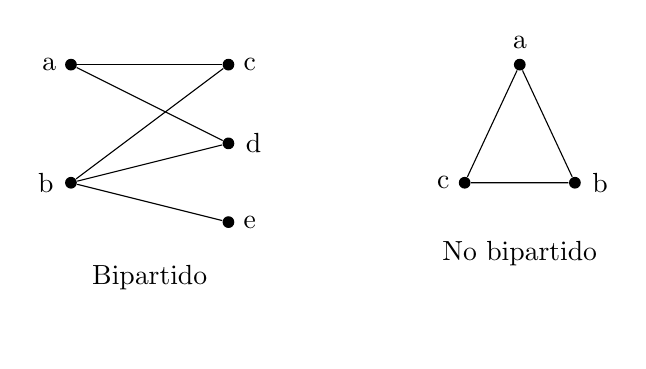
\begin{tikzpicture}[scale=1, every node/.style={circle, fill=black, inner sep=1.5pt}]
\begin{scope}
\node[label=left:{a}] (a) at (0,1.5) {};
\node[label=left:{b}] (b) at (0,0) {};
\node[label=right:{c}] (c) at (2,1.5) {};
\node[label=right:{d}] (d) at (2,0.5) {};
\node[label=right:{e}] (e) at (2,-0.5) {};
\draw (a)--(c);
\draw (a)--(d);
\draw (b)--(c);
\draw (b)--(d);
\draw (b)--(e);
\node[fill=none] at (1,-1.2) {Bipartido};
\end{scope}

\begin{scope}[xshift=5cm]
\node[label=above:{a}] (a2) at (0.7,1.5) {};
\node[label=left:{c}] (c2) at (0,0) {};
\node[label=right:{b}] (b2) at (1.4,0) {};
\draw (a2)--(c2)--(b2)--(a2);
\node[fill=none] at (0.7,-0.9) {No bipartido};
\end{scope}
\end{tikzpicture}
\caption{Cuando $k=2$ el grafo $G$ es llamado \textbf{bipartido}.}
\label{fig:bipartido}
\end{figure}

\begin{ejemplo}
La siguiente figura muestra un grafo 3-partido (nodos $a,b$; $c,d$; $e,f$).
\end{ejemplo}

\begin{ejemplo}[Los puentes de Königsberg]
Durante el siglo \textsc{xvii}, la ciudad de Königsberg (antes en Prusia Oriental; llamada ahora Kaliningrado, en Rusia) estaba dividida en cuatro zonas (incluida la isla de Kneiphof) por el río Pregel. Siete puentes comunicaban estas regiones. Se decía que los habitantes hacían paseos dominicales tratando de encontrar una forma de caminar por la ciudad cruzando cada puente exactamente una vez y regresando al punto donde se había iniciado el paseo. Con el fin de determinar si existía o no dicho circuito, en 1736 el matemático suizo Leonhard Euler representó las cuatro zonas de la ciudad y los siete puentes con el multigrafo correspondiente (ver Figura~\ref{fig:konigsberg}), dando así inicio a la Teoría de Grafos.
\end{ejemplo}

\begin{figure}[htbp]
\centering
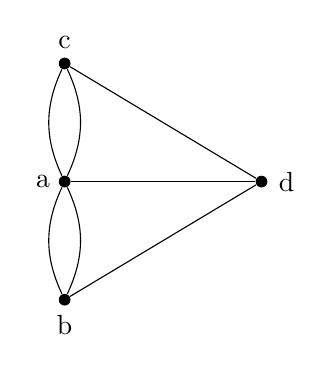
\begin{tikzpicture}[scale=1, every node/.style={circle, fill=black, inner sep=1.5pt}]
\node[label=above:{c}] (c) at (0,1.5) {};
\node[label=left:{a}] (a) at (0,0) {};
\node[label=below:{b}] (b) at (0,-1.5) {};
\node[label=right:{d}] (d) at (2.5,0) {};
\draw (a) to[bend left=25] (c);
\draw (a) to[bend right=25] (c);
\draw (a) to[bend left=25] (b);
\draw (a) to[bend right=25] (b);
\draw (c) -- (d);
\draw (a) -- (d);
\draw (b) -- (d);
\end{tikzpicture}
\caption{Multigrafo que representa los 7 puentes de Königsberg: cuatro zonas (nodos $a,b,c,d$) y siete puentes (aristas).}
\label{fig:konigsberg}
\end{figure}

\section{Representación numérica de los grafos}

Aunque la representación visual de un grafo resulta accesible para el análisis humano, no es viable para su implementación en sistemas computacionales. En consecuencia, se hace imprescindible recurrir a representaciones numéricas que posibiliten el tratamiento automatizado de la información estructural. La literatura ofrece múltiples alternativas para la representación numérica de grafos, cuya idoneidad varía en función del contexto de aplicación. Dichas representaciones pueden estar orientadas a optimizar operaciones de búsqueda y almacenamiento (enfoque algorítmico) o a facilitar el desarrollo de razonamientos de carácter algebraico o combinatorio.

\subsection{Matriz de adyacencia}

Las diversas representaciones matriciales de estructuras de grafo están habitualmente asociadas a la necesidad de realización de cálculos que involucran datos estructurales.

Dado un grafo orientado $G$ con $n$ nodos numerados $v_1, v_2, \ldots, v_n$ (esta numeración define una ordenación arbitraria en el conjunto de nodos) se puede definir la matriz $A$ de orden $n \times n$, donde:
\[
[A]_{ij} =
\begin{cases}
1 & \text{si } (v_i, v_j) \in A \\
0 & \text{si } (v_i, v_j) \notin A
\end{cases}
\]
que denominaremos \textbf{matriz de adyacencia}.

\begin{observacion}
\begin{itemize}
  \item Si un grafo orientado $G$ tiene matriz de adyacencia $A$ entonces $A^T$ es la matriz de adyacencia del dual direccional de $G$.
  \item La matriz de adyacencia de un grafo no orientado se puede representar en su forma triangular (superior o inferior), en vista que no hay distinción entre los dos sentidos posibles para cada arista.
\end{itemize}
\end{observacion}

\begin{ejemplo}
Un dígrafo de 5 nodos con lazos en 1 y 2 tiene matriz de adyacencia:
\[
A =
\begin{bmatrix}
1 & 0 & 0 & 0 & 1 \\
0 & 1 & 1 & 0 & 0 \\
0 & 0 & 0 & 0 & 1 \\
1 & 1 & 0 & 0 & 0 \\
0 & 1 & 0 & 0 & 0
\end{bmatrix}
\]

Un grafo simple de 4 nodos, representado en forma triangular:
\[
A =
\begin{bmatrix}
1 & 0 & 0 & 0 \\
1 & 0 & 0 & 0 \\
0 & 1 & 0 & 0 \\
1 & 0 & 1 & 0
\end{bmatrix}
\]

Un 3-hipergrafo no orientado de 4 nodos, con multiplicidad:
\[
A =
\begin{bmatrix}
1 & 0 & 0 & 0 \\
1 & 0 & 0 & 0 \\
0 & 3 & 0 & 0 \\
0 & 1 & 1 & 0
\end{bmatrix}
\]
\end{ejemplo}

Como limitaciones, cabe observar que esta representación no es adecuada para hipergrafos en general. Con $p$-grafos podrá también haber dificultades: en este caso los valores atribuidos a las posiciones no nulas serán los órdenes de multiplicidad de los arcos o aristas, y la matriz, por tanto, solamente sería formada apenas por valores $0$ y $1$. Tenga presente que mucha de la teoría está basada en la posibilidad de ver la matriz de adyacencia como matriz booleana.

Otra de las desventajas de usar matriz de adyacencia para representar un grafo se debe a que este tipo de representación hace difícil almacenar información adicional acerca del grafo; por ejemplo, si es preciso incluir información acerca de los nodos, será preciso representarla mediante alguna estructura adicional de almacenamiento.

\subsection{Lista de adyacencia}

Esta forma es la más conveniente para la entrada de datos por la simplicidad y ``economía'' de su representación. Es construida como un conjunto de listas de nodos; cada lista está formada por un nodo y por un conjunto de nodos que reciben de él un arco o que con él comparten una arista.

La matriz de adyacencia no es la más ``económica'' de las formas de representación de grafos; ella ocupa $n^2$ posiciones en memoria, en cuanto la lista de adyacencia utiliza apenas $n + m$ posiciones.

\begin{ejemplo}
Para un dígrafo con nodos $\{a,b,c,d,e,f\}$:

\begin{center}
\begin{tabular}{cc}
\begin{tabular}{c|c}
\multicolumn{2}{c}{Nodos} \\
Origen & Destino \\ \hline
a & b \\
b & a c \\
c & a d e f \\
d & a f \\
e & a \\
f & c e
\end{tabular}
&
\begin{tabular}{c|c}
\multicolumn{2}{c}{Nodos} \\
Destino & Origen \\ \hline
a & b c d \\
b & a \\
c & b f \\
d & c \\
e & c f \\
f & c d
\end{tabular}
\end{tabular}
\end{center}
\end{ejemplo}

\section{Relaciones de Adyacencia}

\begin{definicion}
En un grafo orientado $G = (N, A)$ se dice que $y \in N$ es \textbf{sucesor} de $x \in N$, cuando existe $(x,y) \in A$. Una definición dual direccional correspondiente es la de \textbf{antecesor}; luego, habiendo $(x,y) \in A$, $x$ es antecesor de $y$.
\end{definicion}

\begin{definicion}
\textbf{Vecino} o nodo adyacente de un nodo $x$, en un grafo orientado o no, es todo nodo que participa de una conexión con $x$.
\end{definicion}

Los conjuntos de sucesores y de antecesores de un nodo $x$ son denotados, respectivamente, $\Gamma^+(x)$ y $\Gamma^-(x)$, y corresponden a los conjuntos de elementos no nulos de la fila y de la columna asociadas a $x$ en la matriz de adyacencia del grafo. El conjunto de los vecinos de $x \in N$ es denotado $\Gamma(x)$.

\begin{observacion}
\begin{itemize}
  \item La información contenida en los conjuntos de sucesores o antecesores, o de vecinos, equivale a la contenida en el conjunto de conexiones. Por tanto, se puede representar un 1-grafo orientado como $G = (N, \Gamma^+)$ o $G = (N, \Gamma^-)$, y un 1-grafo no orientado por $G = (N, \Gamma)$.
  \item Estos conceptos pueden ser extendidos a subconjuntos de nodos; por ejemplo, si tenemos que $A \subseteq N$:
  \[
  \Gamma^+(A) = \bigcup_{x \in A} \Gamma^+(x)
  \]
  \item Cabe observar que la notación utilizada es abreviada; tratándose, de hecho, de componentes entre conjuntos, la notación correcta es del tipo $\Gamma(\{x\})$.
  \item Las nociones de sucesor y de antecesor pueden ser aplicadas iterativamente, llevando a conceptos que implican la conexión directa o indirecta entre nodos en grafos orientados. Los conjuntos así obtenidos son conocidos como \textbf{clausuras transitivas}.
\end{itemize}
\end{observacion}

\begin{definicion}
Un nodo $y$ es \textbf{alcanzable} a partir de un nodo $x$, cuando existe en el grafo considerado una secuencia de sucesores que se inicia en $x$ y llega a $y$.
\end{definicion}

\begin{definicion}
La \textbf{clausura transitiva directa} $\hat{\Gamma}^+(x)$ de un nodo $x$ es el conjunto de los nodos alcanzables a partir de $x$, y la \textbf{clausura transitiva inversa} $\hat{\Gamma}^-(x)$ de $x$ es el conjunto de los nodos o partes de los cuales $x$ es alcanzable.
\end{definicion}

Estas dos definiciones de clausura son duales direccionales. Es claro que, si $y \in \hat{\Gamma}^+(x)$, $y$ es un \textbf{descendiente} de $x$; si $y \in \hat{\Gamma}^-(x)$, $y$ es un \textbf{ascendiente} de $x$.

\begin{observacion}
Presentamos a continuación el proceso iterativo que conduce a la determinación de $\hat{\Gamma}^+(x)$. Por coherencia con la idea de alcanzable, se acepta al nodo origen como alcanzable a partir de cero etapas:
\[
\Gamma^0(x) = \{x\}, \quad \Gamma^{+1}(x) = \Gamma^+(x), \quad \Gamma^{+2}(x) = \Gamma^+(\Gamma^{+1}(x)), \quad \ldots, \quad \Gamma^{+n}(x) = \Gamma^+(\Gamma^{+n-1}(x))
\]
\[
\hat{\Gamma}^+(x) = \bigcup_{k=0}^{n} \Gamma^{+k}(x)
\]

La noción de clausura transitiva está conceptualmente asociada a las ideas de comunicación y de control. Si definimos un grafo $G = (N, A)$ considerando $N = $ Personas y $A = \{(x,y) \mid x \text{ conoce a } y\}$, la clausura transitiva directa de una persona $k$ será el conjunto de todas las personas que podrán tomar conocimiento de una información que $k$ disponga, a través de comunicación de persona a persona (o sea, sin el uso de los medios de comunicación de masa). La noción puede ser usada, por tanto, para estudiar el efecto de la comunicación informal conocida como ``tele-tipo''.
\end{observacion}

\section{Vecindades de conexiones}

Las definiciones que a continuación se dan son, explícitamente, para grafos sin lazos.

\begin{definicion}
\begin{enumerate}
  \item[a)] Dos conexiones son \textbf{adyacentes} si tienen un nodo en común.
  \item[b)] Se dice que una conexión es \textbf{incidente} en un nodo cuando el nodo forma parte de la conexión. En el caso de grafos orientados, un arco incide exteriormente en $x \in N$ si $x$ es el nodo del cual parte, e incide interiormente en $x$ si $x$ es el nodo al cual llega.
  \item[c)] Para un conjunto de nodos $A \subseteq N$, decimos que un arco incide exterior o interiormente en $A$ si incide de la misma manera en al menos un nodo de $A$.
\end{enumerate}
\end{definicion}

\begin{observacion}
En el caso de grafos no orientados, simplemente se dice que una arista incide en $A \subseteq N$. El conjunto de arcos incidentes exteriormente en $A$ se denota por $\omega^+(A)$, mientras que el conjunto de arcos incidentes interiormente se denota por $\omega^-(A)$; sus cardinalidades son, respectivamente, el \textbf{semigrado exterior} $\delta^+(A)$ y el \textbf{semigrado interior} $\delta^-(A)$.

Para grafos no orientados, el conjunto de aristas incidentes en $A$ se denota simplemente por $\omega(A)$.
\end{observacion}

\begin{ejemplo}
Considere el siguiente grafo no orientado $G = (N,A)$ con nodos $\{1,2,3,4\}$ y aristas $\{1,2\}, \{1,3\}, \{2,4\}, \{3,4\}$.

Tomemos el conjunto de nodos $A = \{1,2\} \subset N$. Las aristas incidentes en $A$ son aquellas que tienen al menos un extremo en $A$:
\[
\omega(A) = \{\{1,2\}, \{1,3\}, \{2,4\}\}
\]
Observe que la arista $\{3,4\}$ no está en $\omega(A)$ porque ninguno de sus extremos pertenece a $A$.

Si el grafo fuera orientado, con arcos $(1,2), (1,3), (2,4), (4,2)$: para el mismo conjunto $A = \{1,2\}$, los conjuntos de arcos incidentes son:
\[
\omega^+(A) = \{(1,2), (1,3)\}
\]
pues estos arcos tienen su extremo inicial en $A$, y
\[
\omega^-(A) = \{(1,2), (4,2)\}
\]
pues estos arcos tienen su extremo final en $A$.

Sus cardinalidades son:
\[
\delta^+(A) = |\omega^+(A)| = 2, \qquad \delta^-(A) = |\omega^-(A)| = 2
\]
Es decir, el semigrado exterior de $A$ es 2 y el semigrado interior de $A$ también es 2.
\end{ejemplo}

\begin{definicion}
El \textbf{grado} $\delta(x)$ de un nodo es el número total de conexiones que en él inciden.
\end{definicion}

\begin{observacion}
\begin{itemize}
  \item En grafos orientados, tenemos evidentemente que $\delta(x) = \delta^+(x) + \delta^-(x)$, y en grafos no orientados $\delta(x) = |\omega(x)|$. Se trata de una definición no orientada válida para $p$-grafos en general.
  \item Un grafo no orientado en el cual $\delta(x) = k$ para todo $x \in N$ es llamado \textbf{regular} (de grado $k$).
  \item Llamamos a un grafo orientado en el cual $\delta^+(x) = k$ ($\delta^-(x) = k$) para todo $x \in N$, \textbf{exteriormente regular} (\textbf{interiormente regular}) (de semigrado $k$).
  \item Para 1-grafos, las cardinalidades de los conjuntos de sucesores (antecesores) de un nodo son iguales a los conjuntos de conexiones exteriormente (interiormente) incidentes que les corresponden.
\end{itemize}
\end{observacion}

\begin{definicion}
Un grafo $G = (N, A)$ será \textbf{completo} si existe al menos una conexión asociada a cada par de nodos.
\end{definicion}

\begin{observacion}
\begin{itemize}
  \item En el caso no orientado significa exactamente una conexión.
  \item El grafo completo poseerá todos los nodos, es decir $G = (N, \mathcal{P}_2(N))$. Evidentemente, todas las estructuras de ese tipo con un mismo orden serán isomorfas; ellas son conocidas como \textbf{grafos completos} y se denotan $K_n$.
  \item Los grafos bipartidos no orientados con el mayor número posible de aristas son llamados \textbf{grafos bipartidos completos} y se denotan con $K_{p,q}$, y el número de aristas será, por tanto, $p \cdot q$.
\end{itemize}
\end{observacion}

\begin{ejemplo}
Los grafos completos $K_1$ a $K_5$ se muestran en la Figura~\ref{fig:completos}.
\end{ejemplo}

\begin{figure}[htbp]
\centering
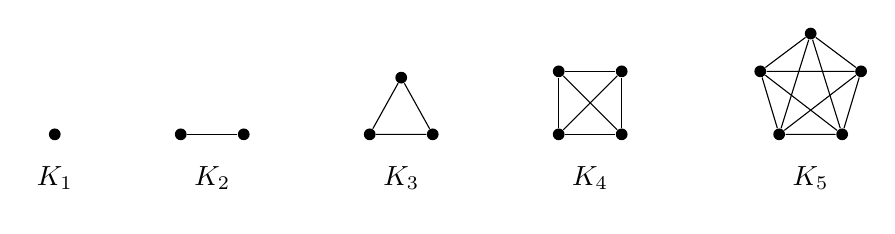
\begin{tikzpicture}[scale=0.8, every node/.style={circle, fill=black, inner sep=1.5pt}]
\begin{scope}
\node (k1) at (0,0) {};
\node[fill=none] at (0,-0.7) {$K_1$};
\end{scope}

\begin{scope}[xshift=2cm]
\node (a) at (0,0) {};
\node (b) at (1,0) {};
\draw (a)--(b);
\node[fill=none] at (0.5,-0.7) {$K_2$};
\end{scope}

\begin{scope}[xshift=5cm]
\node (a) at (0,0) {};
\node (b) at (1,0) {};
\node (c) at (0.5,0.9) {};
\draw (a)--(b)--(c)--(a);
\node[fill=none] at (0.5,-0.7) {$K_3$};
\end{scope}

\begin{scope}[xshift=8cm]
\node (a) at (0,0) {};
\node (b) at (1,0) {};
\node (c) at (1,1) {};
\node (d) at (0,1) {};
\draw (a)--(b)--(c)--(d)--(a);
\draw (a)--(c);
\draw (b)--(d);
\node[fill=none] at (0.5,-0.7) {$K_4$};
\end{scope}

\begin{scope}[xshift=11.5cm]
\node (a) at (0,0) {};
\node (b) at (1,0) {};
\node (c) at (1.3,1) {};
\node (d) at (0.5,1.6) {};
\node (e) at (-0.3,1) {};
\draw (a)--(b) (a)--(c) (a)--(d) (a)--(e);
\draw (b)--(c) (b)--(d) (b)--(e);
\draw (c)--(d) (c)--(e);
\draw (d)--(e);
\node[fill=none] at (0.5,-0.7) {$K_5$};
\end{scope}
\end{tikzpicture}
\caption{Grafos completos $K_1$ a $K_5$.}
\label{fig:completos}
\end{figure}

\begin{definicion}
Dado un grafo $G = (N,A)$, se define su \textbf{grafo complementario} $\overline{G}$ como aquel que tiene el mismo conjunto de nodos $N$ y cuyas conexiones son exactamente aquellas que no están presentes en $G$.

Así, para un grafo orientado:
\[
\overline{G} = (N, N \times N - A)
\]
mientras que para un grafo no orientado:
\[
\overline{G} = (N, \mathcal{P}_2(N) - A)
\]
\end{definicion}

\begin{observacion}
Nótese que el conjunto universal de referencia para las conexiones varía según el tipo de grafo:
\begin{itemize}
  \item En el caso \textbf{no orientado}, dicho universo corresponde al conjunto de todas las aristas posibles, es decir, las aristas de un grafo completo $K_n$.
  \item En el caso \textbf{orientado}, el universo estaría formado por todos los arcos posibles, incluyendo los lazos (es decir, $N \times N$); a este grafo se le denomina \textbf{grafo lleno}.
\end{itemize}

En la práctica es común excluir los lazos en el caso orientado. Bajo este convenio, el universo de referencia para la definición del complemento de un dígrafo es el \textbf{grafo completo simétrico} (aquel que contiene exactamente un arco en cada sentido entre todo par de nodos distintos). En el caso no orientado, la definición también excluye explícitamente los lazos, al tomar como universo $\mathcal{P}_2(N)$ en lugar de $\mathcal{P}(N)$.
\end{observacion}

\section{Trayectoria de un grafo}

\begin{definicion}
Un \textbf{recorrido} o \textbf{itinerario} o \textbf{cadena}, es una familia de conexiones sucesivamente adyacentes.
\end{definicion}

\begin{observacion}
\begin{itemize}
  \item Una cadena será \textbf{cerrada} si la última conexión de la sucesión fuera adyacente a la primera, y \textbf{abierta} en caso contrario. (Una cadena abierta puede contener subtrayectorias cerradas.)
  \item La notación es hecha indicando la sucesión a través de los nodos, las conexiones, o de nodos y conexiones alternados, o apenas los nodos inicial y final, cuando eso fuera suficiente. Por ejemplo, la cadena $\Pi_a$ puede ser expresada de las siguientes formas:
  \begin{align*}
  \Pi_a &= (1,2,3,4,5,3) \\
  \Pi_a &= ((1,2),(2,3),(3,4),(4,5),(5,3)) \\
  \Pi_a &= (1,(1,2),2,(2,3),3,(3,4),4,(4,5),5,(5,3),3) \\
  \Pi_a &= \Pi_{1,3}
  \end{align*}
  \item En un grafo no valorado, el \textbf{tamaño} de una cadena es el número de conexiones por ella utilizadas (contando las repeticiones). Para el caso de grafos valorados, será necesaria la generalización de distancias.
  \item Una cadena es \textbf{simple} si no repite conexiones, y es \textbf{elemental} si no repite nodos. La segunda noción es más restrictiva: toda cadena elemental es simple, pero lo recíproco no es verdadero.
  \item Un \textbf{ciclo} es una cadena simple y cerrada.
  \item Se denomina la \textbf{cintura} $g(G)$ de un grafo al tamaño del menor ciclo que este presente.
  \item Un \textbf{camino} es una cadena en un grafo orientado, en el cual la orientación de los arcos es siempre la misma, a partir del nodo inicial.
  \item Un \textbf{circuito} es un camino simple y cerrado en un grafo orientado.
\end{itemize}
\end{observacion}

\begin{definicion}
\begin{itemize}
  \item Una cadena (abierta o cerrada) se denomina \textbf{euleriana} si recorre cada conexión del grafo exactamente una vez; y se denomina \textbf{hamiltoniana} si visita cada nodo del grafo exactamente una vez.
  \item Si se permite la repetición, la cadena se denomina \textbf{pre-euleriana} o \textbf{pre-hamiltoniana}, según corresponda.
  \item Un grafo se dice \textbf{euleriano} (o \textbf{hamiltoniano}) si posee una cadena cerrada euleriana (o hamiltoniana, respectivamente).
\end{itemize}
\end{definicion}

\begin{ejemplo}[Cadena euleriana y grafo euleriano]
Considere el siguiente grafo no dirigido con nodos $A, B, C, D$ y ocho aristas entre ellos. Una cadena euleriana para este grafo es:
\[
A \to B \to D \to A \to C \to D \to B \to C \to A
\]
Esta cadena recorre cada una de las 8 aristas exactamente una vez y regresa al nodo inicial, por lo que es un \textbf{ciclo euleriano}. En consecuencia, el grafo es euleriano.
\end{ejemplo}

\begin{ejemplo}[Cadena hamiltoniana y grafo hamiltoniano]
Considere el siguiente grafo con nodos $A, B, C, D, E$. Una cadena hamiltoniana para este grafo es:
\[
A \to B \to C \to D \to E \to A
\]
Esta cadena visita cada uno de los 5 nodos exactamente una vez y regresa al nodo inicial, por lo que es un \textbf{ciclo hamiltoniano}. En consecuencia, el grafo es hamiltoniano.
\end{ejemplo}

\section{Grafos conexos -- Componentes f-conexas}

El concepto de conexidad está relacionado a la posibilidad de llegar de un nodo a otro en un grafo a través de las conexiones existentes. Esto es, el estado de conexión de un grafo adquiere aspectos diferentes conforme el grafo sea orientado o no. La idea de llegar está relacionada con la definición de alcanzable, la cual puede ser usada con interés, especialmente en grafos orientados.

\begin{definicion}
Un grafo (orientado o no) es \textbf{conexo} si para cualquier pareja de nodos del grafo se puede llegar al otro nodo partiendo de cualquiera de ellos.
\end{definicion}

\begin{definicion}
Un dígrafo en el cual todo par de nodos es unido por al menos una cadena se denomina \textbf{simplemente conexo} o \textbf{s-conexo}.
\end{definicion}

\begin{definicion}
Un dígrafo en el cual, en todo par de nodos, al menos uno es alcanzable a partir del otro, se denomina \textbf{semi-fuertemente conexo} o \textbf{sf-conexo}.
\end{definicion}

\begin{definicion}
Un dígrafo en el cual toda pareja de nodos son mutuamente alcanzables se denomina \textbf{fuertemente conexo} o \textbf{f-conexo}.
\end{definicion}

\begin{observacion}
\begin{enumerate}
  \item[a)] De las definiciones anteriores se desprende que todo dígrafo fuertemente conexo (f-conexo) es también semi-fuertemente conexo (sf-conexo) y, por tanto, simplemente conexo (s-conexo). Análogamente, todo dígrafo semi-fuertemente conexo es también simplemente conexo. Esta jerarquía permite establecer la siguiente clasificación, que constituye una partición del conjunto de todos los dígrafos:
  \begin{itemize}
    \item $C_3$ = dígrafos que son f-conexos
    \item $C_2$ = dígrafos que son sf-conexos y que no son f-conexos
    \item $C_1$ = dígrafos que son s-conexos y que no son sf-conexos
    \item $C_0$ = dígrafos que no son s-conexos
  \end{itemize}
  \item[b)] Las propiedades de los dígrafos de las categorías $C_1$ y $C_2$ ameritan una discusión en detalle por el interés en la presencia, en esos casos, de nodos privilegedos. La discusión de $C_3$ está asociada con el concepto de conexidad.
  \item[c)] Para un dígrafo $G$ y su complemento $\overline{G}$, se tiene:
  \begin{align*}
  G \in C_0 &\;\Rightarrow\; \overline{G} \in C_3 \\
  G \in C_1 \;\;\text{o}\;\; G \in C_2 \\
  G \in C_3 &\;\Rightarrow\; \overline{G} \notin C_i, \quad i = 0,1,2,3
  \end{align*}
\end{enumerate}
\end{observacion}

\begin{observacion}
La f-conexidad se caracteriza por la alcanzabilidad recíproca entre nodos, lo que convierte a la relación de alcanzabilidad en una relación simétrica. Además, todo nodo es alcanzable desde sí mismo (reflexividad), y si $z$ es alcanzable desde $y$, e $y$ es alcanzable desde $x$, entonces $z$ es alcanzable desde $x$ (transitividad). Por tanto, la relación de alcanzabilidad en un dígrafo $G = (N, A)$ es una relación de equivalencia sobre $N$, y en consecuencia induce una partición $S = \{S_1, S_2, \ldots, S_\gamma\}$ del conjunto de nodos. Los subgrafos inducidos por cada $S_i$ reciben el nombre de \textbf{componentes f-conexas maximales} o, simplemente, \textbf{componentes f-conexas}. Si el dígrafo es f-conexo, la partición consta de un único elemento: $S = \{N\}$.

La relación de sf-conexidad no es reflexiva; por tanto, las componentes sf-conexas no corresponden a una partición del conjunto de nodos $N$.
\end{observacion}

\section{Algunos resultados}

\begin{teorema}[Lema del apretón de manos]
Si $G = (N, A)$ es un multigrafo entonces
\[
\sum_{v \in N} \delta(v) = 2|A|
\]
\end{teorema}

\begin{proof}
Al considerar cada arista $\{a,b\}$ del grafo $G$ encontramos que la arista contribuye con una unidad a $\delta(a)$ y a $\delta(b)$, y en consecuencia, con dos unidades a $\sum_{v \in N} \delta(v)$. Así,
\[
\sum_{v \in N} \delta(v) = 2|A|. \qedhere
\]
\end{proof}

\begin{corolario}
Para cualquier multigrafo, el número de nodos de grado impar debe ser par.
\[
\sum_{\text{Par}} \delta(v) + \sum_{\text{Impar}} \delta(v) = 2|A|
\]
\end{corolario}

\begin{ejemplo}
¿Es posible tener un grafo 4-regular con 10 aristas?

\textbf{Solución.} De acuerdo con el teorema del apretón de manos, se tiene que:
\[
\sum_{v \in N} \delta(v) = 2|A|
\]
Si el grafo es 4-regular, entonces $\delta(v) = 4$ para todo $v \in N$. Por lo tanto:
\[
\sum_{v \in N} \delta(v) = 4|N|
\]
Sustituyendo en la fórmula:
\[
4|N| = 2(10) = 20 \quad\Longrightarrow\quad |N| = \frac{20}{4} = 5
\]
Por lo tanto, el grafo solicitado debe tener 5 nodos. Un ejemplo de tal grafo es el grafo completo $K_5$, que tiene 5 nodos y cada nodo tiene grado 4. El número de aristas de $K_5$ es:
\[
|A| = \binom{5}{2} = \frac{5 \cdot 4}{2} = 10
\]
Efectivamente, $K_5$ es un grafo 4-regular con 10 aristas.

\textbf{Respuesta:} Sí, es posible. El grafo $K_5$ cumple con las condiciones requeridas.
\end{ejemplo}

\begin{teorema}
En un dígrafo $G = (N,A)$, todo nodo del dígrafo se encuentra exactamente en una componente fuerte.
\end{teorema}

\begin{proof}
Las componentes f-conexas son subgrafos definidos en algún elemento de la partición definida por la relación de alcanzabilidad en $N$, es decir, que todo nodo del dígrafo se encuentra exactamente en una componente f-conexa.
\end{proof}

\begin{teorema}
Sea $G = (N,A)$ un grafo o multigrafo no dirigido sin nodos aislados. Entonces $G$ tiene un ciclo euleriano si y solo si $G$ es conexo y todo nodo de $G$ tiene grado par.
\end{teorema}

\begin{proof}
$(\Rightarrow)$ Sea $G$ euleriano. Entonces existe un ciclo que pasa por todo nodo $v \in N$; entonces, para un par de nodos cualesquiera $x$ e $y$, existe una cadena simple que puede llegar de $x$ a $y$; por tanto, $G$ es conexo. Por otro lado, al intentar recorrer el ciclo euleriano podremos escoger un nodo y de ahí proseguir atravesando los demás nodos, borrando las aristas utilizadas; al atravesar un nodo $x$, su grado $\delta(x)$ disminuirá en dos unidades; luego, todos los nodos intermediarios en la cadena deberán tener grado par, o será imposible anular todos sus grados al final de este proceso. El nodo inicial también deberá tener grado par, en vista que el uso de una de sus aristas adyacentes al inicio lo dejará con grado inicialmente impar, lo que permitirá su anulación al final del proceso.

$(\Leftarrow)$ Sea $G$ conexo, con todos sus nodos de grado par. Procederemos por inducción en el número de aristas. Si el número de aristas de $G$ es 1 o 2, entonces $G$ debe ser un ciclo, que evidentemente son eulerianos.

Ahora supongamos que $G$ es euleriano para cuando hay menos de $n$ aristas. Luego, si $G$ tiene $n$ aristas, seleccionamos un nodo $c$ en $G$ como punto inicial para construir un ciclo euleriano. Como $G$ es conexo y cada nodo tiene grado par, existe al menos un ciclo $\ell$ que contenga a $c$. Si $\ell$ tiene todas las aristas de $G$, hemos terminado. Si no, eliminamos las aristas del ciclo $\ell$ en $G$, asegurándonos de eliminar cualquier nodo que haya quedado aislado. El subgrafo restante $K$ tiene todos los nodos de grado par. Si $K$ es conexo, hemos terminado. Si $K$ no es conexo, cada componente de $K$ es conexa y tendrá un ciclo euleriano.

Además, cada uno de estos ciclos eulerianos tiene un nodo que está en $\ell$. En consecuencia, podemos partir de $c$ y recorrer $\ell$ hasta llegar al nodo $c_1$ que está en el ciclo euleriano de una componente de $K$; entonces se recorre este ciclo euleriano y, al regresar a $c_1$, continuamos en $\ell$ hasta llegar a un nodo $c_2$ que está en el ciclo euleriano de la otra componente de $K$. Como el grafo $G$ es finito, podemos continuar este proceso hasta construir un ciclo euleriano para $G$.
\end{proof}

\begin{corolario}
Si $G$ es un grafo o multigrafo no dirigido sin nodos aislados, entonces podemos construir una cadena abierta euleriana en $G$ si y solo si $G$ es conexo y tiene exactamente dos nodos de grado impar.
\end{corolario}

\begin{proof}
Si $G$ es conexo y $x$ e $y$ son los nodos de $G$ de grado impar, añadimos una arista $\{x,y\}$ a $G$. Ahora tenemos un grafo $G$ conexo tal que todos sus nodos son de grado par. Por lo tanto, $G$ tiene un ciclo euleriano $C$; cuando eliminamos la arista $\{x,y\}$ de $C$, obtenemos una cadena abierta euleriana de $x$ a $y$ en $G$. Lo recíproco se deja como tarea.
\end{proof}

\begin{ejemplo}[Aplicación del Teorema de Euler: el problema de los puentes de Königsberg]
Los habitantes se preguntaban si era posible realizar un recorrido que cruzara cada puente exactamente una vez y regresara al punto de partida. En términos de teoría de grafos, la pregunta equivale a determinar si este multigrafo (Figura~\ref{fig:konigsberg}) tiene un \textbf{ciclo euleriano}.

Aplicando el Teorema de Euler, debemos verificar dos condiciones:

\begin{enumerate}
  \item \textbf{El grafo debe ser conexo.} En efecto, el multigrafo que modela la ciudad es conexo, ya que es posible ir de cualquier zona a cualquier otra a través de los puentes.
  \item \textbf{Todos los nodos deben tener grado par.} Calculemos los grados de cada nodo:
  \[
  \delta(a) = 5, \quad \delta(b) = 3, \quad \delta(c) = 3, \quad \delta(d) = 3
  \]
\end{enumerate}

Observamos que todos los nodos tienen grado \textbf{impar}. Por lo tanto, el multigrafo \textbf{no satisface} la segunda condición del teorema. En consecuencia, no existe un ciclo euleriano que recorra cada puente exactamente una vez y regrese al punto de inicio.

Euler demostró que, para que tal recorrido sea posible, todos los nodos deben tener grado par, condición que no se cumple en este caso. Así quedó establecido que el paseo soñado por los habitantes de Königsberg era imposible, dando origen a la teoría de grafos.

\textbf{Nota:} si el objetivo hubiera sido un recorrido que cruzara cada puente exactamente una vez sin necesidad de regresar al punto de partida (camino euleriano abierto), el teorema establece que el grafo debe tener exactamente dos nodos de grado impar. En este caso, hay cuatro nodos de grado impar, por lo que tampoco existe un camino euleriano abierto.
\end{ejemplo}

\begin{corolario}
Sea $G = (N,A)$ un grafo o multigrafo dirigido sin nodos aislados. El grafo $G$ tiene un circuito euleriano dirigido si y solo si $G$ es conexo y $\delta^+(x) = \delta^-(x)$ para todo $x \in N$.
\end{corolario}

\begin{ejemplo}[Aplicación de circuitos eulerianos: generación de secuencias binarias]
Se muestra la superficie de un disco de rotación dividido en ocho sectores de igual área, con material conductor y no conductor colocado en el disco.

Cuando las tres terminales hacen contacto con tres sectores dados, el material no conductor produce un flujo de corriente y aparece un 1 en la pantalla de un dispositivo digital. Para los sectores con material conductor, se produce un flujo de corriente y aparece un 0 en la pantalla. Si el disco se rota 45 grados (en sentido de las manecillas del reloj), en la pantalla se leería 110 (de arriba a abajo). Así, podemos obtener al menos dos (100 y 110) de las ocho representaciones binarias del 0 al 7.

La pregunta es: ¿podemos representar los ocho números binarios al rotar el disco? Para responder esta pregunta, se construye un dígrafo $G = (N,A)$ donde
\[
N = \{00, 01, 10, 11\}
\]
y $A$ se construye como sigue: si $b_1b_2, b_2b_3 \in N$, entonces $(b_1b_2, b_2b_3) \in A$. Esto produce un dígrafo con lazos en $00$ y $11$, y arcos entre $00-01$, $01-10$ (doble), $01-11$, $10-00$, $10-11$.

Se observa que este dígrafo es conexo y que, para todo $x \in N$, $\delta^+(x) = \delta^-(x)$. Por el corolario anterior, se tiene un circuito euleriano:
\[
10 \to 00 \to 00 \to 01 \to 10 \to 01 \to 11 \to 11 \to 10
\]

Al etiquetar cada arco $a = (x,y)$ con la sucesión de tres bits $b_1b_2b_3$, donde $x = b_1b_2$ e $y = b_2b_3$, se determinan las ocho sucesiones de tres bits distintas. Así mismo, cualesquiera dos etiquetas de arcos consecutivos en el circuito euleriano son de la forma $b_1b_2b_3$ y $b_2b_3b_4$.

Partiendo del arco con etiqueta $100$, a fin de obtener la siguiente etiqueta ($000$), concatenamos el último bit de $000$, es decir $0$, a la cadena $100$. Entonces, la cadena resultante $1000$ proporciona $100$ ($100|0$) y $000$ ($1|000$). La siguiente etiqueta de arco es $001$, por lo que concatenamos el $1$ (el último bit de $001$) y obtenemos $10001$, lo cual proporciona las tres sucesiones de tres bits distintas: $100$ ($100|01$), $000$ ($1|000|1$) y $001$ ($10|001$). Continuando de esta forma llegamos a la sucesión de ocho bits:
\[
10001011
\]
(donde el último 1 se envuelve), y estos ocho bits se acomodan en los sectores del disco giratorio.

A partir de esta configuración, al rotar el disco, se obtienen las ocho sucesiones de tres bits:
\[
100,\ 110,\ 111,\ 011,\ 101,\ 010,\ 001,\ 000
\]
que corresponden a todas las representaciones binarias del 0 al 7.

Así, mediante el uso de un circuito euleriano en el dígrafo construido, se logra representar todos los números binarios del 0 al 7 al rotar el disco.
\end{ejemplo}

\subsection{Algoritmo de Fleury}

El algoritmo de Fleury obtiene un ciclo de Euler para un grafo conexo sin nodos de grado impar.

Una arista $\{x,y\}$ es un \textbf{puente} en un grafo conexo $G$ si al eliminar $\{x,y\}$ se crea un grafo disconexo.

Sea $G = (N,A)$ un grafo conexo con todos sus nodos de grado par.

\begin{algorithm}[htbp]
\caption{Algoritmo de Fleury}
\begin{algorithmic}[1]
\Require Un grafo conexo $G = (N,A)$ con todos sus nodos de grado par
\Ensure Un ciclo euleriano $\pi$
\State Elegir un nodo $v \in N$ como nodo inicial para el ciclo
\State $\pi \gets (v)$
\While{existan aristas en $A$}
  \State Suponer que ya se ha construido $\pi = (v, u, \ldots, w)$
  \If{en $w$ solo existe una arista $\{w,z\}$}
    \State Extender $\pi$ a $\pi = (v, u, \ldots, w, z)$
    \State Eliminar $\{w,z\}$ de $A$ y eliminar $w$ de $N$ si queda aislado
  \Else
    \State Elegir una arista $\{w,z\}$ que no sea un puente
    \State Extender $\pi$ a $\pi = (v, u, \ldots, w, z)$
    \State Eliminar $\{w,z\}$ de $A$
  \EndIf
\EndWhile
\State \Return $\pi$
\end{algorithmic}
\end{algorithm}

\subsection{Caminos Hamiltonianos}

Con respecto a las cadenas hamiltonianas surgen preguntas análogas a las correspondientes eulerianas. ¿Es posible determinar si existe una cadena hamiltoniana? Y si existe, ¿hay una manera eficiente de determinarla? Puede parecer sorprendente, pero la primera pregunta no ha sido resuelta de manera completa hasta la fecha. Sin embargo, daremos algunos resultados.

Es claro que los lazos y las aristas múltiples no son muy útiles para determinar las cadenas hamiltonianas, ya que entre dos nodos solo puede utilizarse una arista. También es fácil verificar que si un grafo $G$ de $n$ nodos tiene un ciclo hamiltoniano, entonces $G$ debe tener al menos $n$ aristas.

\begin{teorema}
Sea $G = (N,A)$ un grafo sin lazos, con $|N| = n \geq 2$. Si $\delta(x) + \delta(y) \geq n-1$ para todos $x, y \in N$, $x \neq y$, entonces $G$ tiene una cadena abierta hamiltoniana.
\end{teorema}

\begin{corolario}
Sea $G = (N,A)$ un grafo sin lazos, con $|N| = n \geq 2$. Si $\delta(x) \geq \dfrac{n-1}{2}$, $\forall x \in N$, entonces $G$ tiene una cadena abierta hamiltoniana.
\end{corolario}

\begin{teorema}
Sea $G = (N,A)$ un grafo sin lazos, con $|N| = n \geq 3$. Si $\delta(x) + \delta(y) \geq n$ para todos $x, y \in N$ no adyacentes, entonces $G$ tiene un ciclo hamiltoniano.
\end{teorema}

\begin{corolario}
Si $G = (N,A)$ es un grafo sin lazos, con $|N| = n \geq 3$ y si $\delta(x) \geq \dfrac{n}{2}$ para todo $x \in N$, entonces $G$ tiene un ciclo hamiltoniano.
\end{corolario}

\begin{corolario}
Si $G = (N,A)$ es un grafo sin lazos, con $|N| = n \geq 3$ y $|A| \geq \dfrac{1}{2}(n^2 - 3n + 6)$, entonces $G$ tiene un ciclo hamiltoniano.
\end{corolario}

Los recíprocos de los resultados anteriores no son válidos; es decir, las condiciones dadas son suficientes, pero no necesarias, para la conclusión.

El problema que se ha considerado tiene algunas variantes importantes. En un caso, las aristas pueden tener valores que representen una distancia, un costo o algo similar. Entonces el problema es determinar un ciclo hamiltoniano tal que la suma total de valores en la cadena sea mínima. Por ejemplo, los nodos podrían representar ciudades; las aristas, líneas de transporte; y el valor de una arista, el costo del viaje. Esta versión del problema se conoce como el \textbf{problema del agente viajero}.

\section{Un modelo de administración de proyectos}

En la década de 1950 aparecieron dos enfoques básicos para la planificación temporal, planteamiento y control de proyectos: PERT (\emph{Program Evaluation and Review Technique} o Técnica de Evaluación y Revisión de Programas) y CPM (\emph{Critical Path Method} o Método del camino crítico). Aunque en un principio existían diferencias fundamentales entre los dos métodos, el subsiguiente desarrollo de estos métodos ha disipado esas diferencias. Consiguientemente, en lo que sigue no se distingue entre PERT y CPM.

La construcción de una red de planificación temporal está limitada por las reglas siguientes:

\begin{itemize}
  \item Toda actividad debe ser representada por un único arco (esto es, las actividades son únicas).
  \item Como máximo, una actividad puede salir de un nodo y terminar en otro (esto es, el grafo es simple).
\end{itemize}

La segunda regla obliga al uso de \textbf{actividades mudas}. Una actividad muda no requiere tiempo alguno para su terminación, pero se necesita porque el grafo debe ser simple, y es necesario modelar ciertas relaciones lógicas.

El objetivo principal de la administración de proyectos es determinar el camino crítico y producir una planificación temporal que muestre los instantes de comienzo y finalización para todas las actividades de la red. Para la determinación de estas actividades temporales resultan útiles los siguientes conceptos:

\begin{definicion}
El \textbf{instante mínimo de comienzo}, $TE_j$, para cada suceso $j$, es el primer momento en que puede producirse ese suceso de tal manera que ya hayan finalizado todas las actividades entrantes de ese suceso.
\end{definicion}

El valor $TE_j$ de cada suceso se genera efectuando una pasada hacia adelante en la red, desde la fuente hasta el sumidero. En términos de la red, esto corresponde a la asignación de valores temporales a cada nodo (o suceso), de tal forma que el valor que se asigna a cada suceso es la cantidad de tiempo necesaria para completar las actividades presentes a lo largo del camino más largo que lleve a ese suceso.

Por definición, a la fuente se le asocia el valor cero. En general, el instante mínimo para un suceso está dado por una longitud máxima desde la fuente hasta el suceso.
\[
TE_1 = 0, \qquad TE_j = \max\{TE_i + t_{ij}\}, \quad j \neq 1
\]
para todas las posibles actividades que entren en el suceso $j$.

\begin{definicion}
El \textbf{tiempo máximo de finalización}, $TL_i$, es el último momento en que puede producirse un suceso sin dar lugar a un retraso del proyecto.
\end{definicion}

El valor de $TL_i$ para cada suceso se calcula efectuando una pasada hacia atrás desde el sumidero hacia la fuente.

El tiempo máximo de finalización asociado a cada suceso es el último momento en que puede finalizar una actividad sin dar lugar a un retraso en la fecha mínima de finalización del proyecto (esto es, son los tiempos finales de terminación asociados a aquellas actividades que no dan lugar a que aumente el valor $TE$ del nodo sumidero).

En general, el tiempo máximo de finalización para cualquier suceso se puede calcular de la siguiente manera:
\[
TL_s = TE_s, \qquad TL_i = \min\{TL_j - t_{ij}\}, \quad i \neq s
\]
donde $s$ es el sumidero. Es preciso tomar el mínimo porque al satisfacer la fecha final más temprana también se satisfacen las posteriores.

\section{Ejercicios}

\begin{ejercicio}
Los turistas Jenssen, Leuzinger, Dufour y Medeiros se encuentran en un bar de París y comienzan a conversar. Las lenguas disponibles son el inglés, el francés, el portugués y el alemán; Jenssen habla todas, Leuzinger no habla apenas el portugués, Dufour habla francés y alemán y Medeiros habla inglés y portugués.
\begin{enumerate}
  \item[a)] Represente por medio de un grafo $G = (N, A)$ todas las posibilidades de que uno de ellos dirija la palabra a otro, siendo comprendido. Defina $N$ y $A$.
  \item[b)] Represente por medio de un hipergrafo $H = (N, A')$ las capacidades lingüísticas del grupo. ¿Cuál es el significado de las intersecciones $a_i \cap a_j$ donde los $a_k \in A'$?
\end{enumerate}
\end{ejercicio}

\begin{ejercicio}
La figura muestra un grafo no dirigido que representa una sección de unos grandes almacenes. Los nodos indican el lugar donde se localizan las cajas; las aristas indican los pasillos que hay entre ellas. Los almacenes necesitan instalar un sistema de seguridad que consiste en colocar guardias (vestidos de civil) en ciertas cajas, de manera que cada cajero tenga un guardia en su lugar o que haya un solo pasillo entre una caja con guardia y el cajero. ¿Cuál es el número mínimo de guardias necesarios?
\end{ejercicio}

\begin{ejercicio}
Mostrar que los grafos dados son isomorfos.
\end{ejercicio}

\begin{ejercicio}
Mostrar que los dígrafos dados son isomorfos.
\end{ejercicio}

\begin{ejercicio}
Mostrar que los dígrafos dados no son isomorfos.
\end{ejercicio}

\begin{ejercicio}
Cada uno de los siguientes multigrafos surge en el análisis de un conjunto de cuatro bloques para el juego de ``locura instantánea''. Determine en cada caso si es posible resolver el acertijo.
\end{ejercicio}

\begin{ejercicio}
Diga si los dos grafos presentados son o no isomorfos. Si lo fueran, presente la función que establece el isomorfismo entre ellos; caso contrario, explique por qué.
\end{ejercicio}

\begin{ejercicio}
Escriba la matriz de adyacencia que representa a los siguientes grafos.
\end{ejercicio}

\begin{ejercicio}
Describa la matriz de adyacencias para $K_n$.
\end{ejercicio}

\begin{ejercicio}
Dada una matriz de adyacencias $A$ para un grafo simple $G$, describa la matriz de adyacencia para el complemento $\overline{G}$.
\end{ejercicio}

\begin{ejercicio}
Para el ejercicio 8, diseñe la representación en la forma de lista de adyacencias para el grafo indicado.
\end{ejercicio}

\begin{ejercicio}
Diseñe una representación en forma de matriz de incidencia para el grafo valorado de la figura.
\end{ejercicio}

\begin{ejercicio}
¿Cuál es el número total de aristas en $K_n$? Justifique su respuesta.
\end{ejercicio}

\begin{ejercicio}
¿Cuál es el grado de cada nodo de $K_n$?
\end{ejercicio}

\begin{ejercicio}
Si $G_1$ y $G_2$ son grafos no dirigidos (sin lazos), demuestre que $G_1, G_2$ son isomorfos si y solo si $\overline{G_1}$ y $\overline{G_2}$ son isomorfos. Determine si los siguientes grafos son isomorfos.
\end{ejercicio}

\begin{ejercicio}
Sea un grafo no dirigido con $n$ nodos. Si $G$ es isomorfo a su propio complemento $\overline{G}$ (este grafo se conoce como \textbf{autocomplementario}), ¿cuántas aristas debe tener $G$? Encuentre un ejemplo de un grafo autocomplementario con cuatro nodos y otro con cinco nodos. Si $G$ es un grafo autocomplementario con $n$ nodos, donde $n > 1$, demuestre que $n = 4k$ o $n = 4k+1$, para alguna $k \in \Z^+$.
\end{ejercicio}

\begin{ejercicio}
Sea $G$ un ciclo con $n$ nodos. Demuestre que $G$ es autocomplementario si y solo si $n = 5$.
\end{ejercicio}

\begin{ejercicio}
Dar tres caminos elementales que vayan de 1 a 3 para el dígrafo dado. ¿Existe algún circuito en el dígrafo? ¿Es transitivo el dígrafo?
\end{ejercicio}

\begin{ejercicio}
Calcular todos los semigrados exterior e interior de los nodos del dígrafo dado. Dar todos los circuitos elementales de este grafo. Obtener un dígrafo que no presente ningún circuito eliminando una arista del dígrafo dado. Determinar todos los nodos que puedan alcanzar cualquier otro nodo del dígrafo.
\end{ejercicio}

\begin{ejercicio}
Para los dígrafos dados en los ejercicios 18 y 19, determinar si son fuertemente conexos, semi-fuertemente conexos o simplemente conexos.
\end{ejercicio}

\begin{ejercicio}
Demostrar que un dígrafo $G$ es fuertemente conexo si y solo si existe un circuito en $G$ que incluye a todos los nodos al menos una vez.
\end{ejercicio}

\begin{ejercicio}
Hallar las componentes f-conexas del dígrafo dado en el problema 19. Calcular también sus componentes.
\end{ejercicio}

\begin{ejercicio}
El dígrafo de abajo representa las respuestas a la pregunta: ``¿Cuáles son los colegas de quien Ud. más gusta?'' dadas por una promoción de primer semestre de estudiantes de la UNSA (un grafo como este es denominado \textbf{sociograma}). Use notación y nomenclatura convenientes para indicar la existencia de líder(es), amistades recíprocas, problemas de relacionamiento, influencias directas o indirectas y aislamiento.
\end{ejercicio}

\begin{ejercicio}
Un museo de arte ha ordenado la exposición que actualmente presenta en cinco salas, como muestra la figura. ¿Existe alguna forma de recorrer la exposición de modo que Ud. pase por cada puerta solo una vez? En este caso, trace el recorrido.
\end{ejercicio}

\begin{ejercicio}
En la puerta de una mansión histórica, usted recibe una copia del plano de la casa. ¿Es posible visitar cada cuarto de la casa pasando por cada puerta solo una vez? Explique el razonamiento.
\end{ejercicio}

\begin{ejercicio}
Trace $K_{2,3}$, $K_{2,4}$, $K_{3,3}$.
\end{ejercicio}

\begin{ejercicio}
Obtenga una fórmula para el número de aristas de $K_{m,n}$.
\end{ejercicio}

\begin{ejercicio}
¿Para qué valores de $m$ y $n$ tiene $K_{m,n}$ un circuito euleriano?
\end{ejercicio}

\begin{ejercicio}
Diseñe un juego de ``locura instantánea'' que tenga exactamente cuatro soluciones.
\end{ejercicio}

\begin{ejercicio}
En el siguiente grafo, los nodos representan ciudades y los números de las aristas señalan los costos de construcción de la carretera correspondiente. Determine un sistema de caminos de menor costo que conecte todas las ciudades. ¿Es esta una solución única?
\end{ejercicio}

\begin{ejercicio}
Suponga que un grafo tiene una matriz de adyacencia de la forma
\[
A =
\begin{bmatrix}
A' & 0 \\
0 & A''
\end{bmatrix}
\]
en donde los elementos fuera de las submatrices $A'$ y $A''$ son ceros. ¿Cómo debe ser el esquema del grafo?
\end{ejercicio}

\begin{ejercicio}
Demuestre que un camino que no es simple debe contener un circuito.
\end{ejercicio}

\begin{ejercicio}
Demuestre que si $G'$ es un subgrafo conexo de un grafo $G$, entonces $G'$ está contenido en un componente de $G$.
\end{ejercicio}

\begin{ejercicio}
Todo nodo y toda arista de un dígrafo están contenidos en una componente s-conexa y en solo una.
\end{ejercicio}

\begin{ejercicio}
Demostrar el Corolario 5.36.
\end{ejercicio}

\begin{ejercicio}
Determine los valores de $n$ para los que el grafo completo $K_n$ tiene ciclo euleriano. ¿Para cuáles $n$ tiene $K_n$ una cadena abierta euleriana pero no un ciclo euleriano?
\end{ejercicio}

\begin{ejercicio}
Diga si es posible trazar la figura sin levantar el lápiz. Explique su razonamiento.
\end{ejercicio}

\begin{ejercicio}
Sea $N = \{000, 001, 010, \ldots, 111\}$. Para cualquier sucesión de cuatro bits $b_1, b_2, b_3, b_4$, trace una arista del elemento $b_1b_2b_3$ al elemento $b_2b_3b_4$ en $N$.
\begin{enumerate}
  \item[a)] Trace el grafo $G = (N,A)$ descrito.
  \item[b)] Encuentre un ciclo euleriano para $G$.
  \item[c)] Distribuya ocho ceros y ocho unos de modo uniforme alrededor del borde de un disco que gira en el sentido de las manecillas del reloj, de modo que estos 16 bits formen una sucesión circular tal que las subsucesiones (consecutivas) de longitud 4 proporcionen las representaciones binarias de $0,1,2,3,\ldots,15$ en algún orden.
\end{enumerate}
\end{ejercicio}

\begin{ejercicio}
Determine $|N|$ para los siguientes grafos o multigrafos $G$:
\begin{enumerate}
  \item[a)] $G$ tiene nueve aristas y todos los nodos tienen grado 3.
  \item[b)] $G$ es regular con 15 aristas.
  \item[c)] $G$ tiene 10 aristas con dos nodos de grado 4 y los demás de grado 3.
\end{enumerate}
\end{ejercicio}

\begin{ejercicio}
Si $G = (N,A)$ es un grafo conexo con $|A| = 17$ y $\delta(x) \geq 3$ para todo $x \in N$, ¿cuál es el valor máximo para $|N|$?
\end{ejercicio}

\begin{ejercicio}
Sea $N = \{a,b,c,d,e,f\}$. Dibuje tres grafos sin lazos en los que $\delta(a) = 3$, $\delta(b) = \delta(c) = 2$ y $\delta(d) = \delta(e) = \delta(f) = 1$. ¿Cuántos de esos grafos son conexos?
\end{ejercicio}

\begin{ejercicio}
Dé un ejemplo de un grafo conexo tal que:
\begin{enumerate}
  \item[a)] No tenga ciclos eulerianos ni ciclos hamiltonianos.
  \item[b)] Tenga un ciclo euleriano pero no un ciclo hamiltoniano.
  \item[c)] Tenga un ciclo hamiltoniano pero no un ciclo euleriano.
  \item[d)] Tenga un ciclo hamiltoniano y un ciclo euleriano.
\end{enumerate}
\end{ejercicio}

\begin{ejercicio}
Determine si el grafo dado tiene un ciclo hamiltoniano, una cadena hamiltoniana pero no un ciclo hamiltoniano, o ninguno de los dos. Si el grafo tiene un ciclo hamiltoniano, indique el ciclo.
\end{ejercicio}